
\documentclass[12pt]{article}
\usepackage{caption}
\usepackage[utf8]{inputenc}
\usepackage{graphicx}
\usepackage{amsmath}
\usepackage{float}
\usepackage{hyperref}
\usepackage{geometry}
\geometry{margin=1in}
\title{Análisis del arituclo Market Efficiency During the COVID-19 Pandemic. Some
Insights Using Non-Parametric Tests }
\author{B. Barreto, M. Ramos, E. Navarrete}
\date{20 de mayo de 2025}

\begin{document}

\maketitle

\section{Introducción}
Este informe tiene como objetivo comparar el análisis realizado por Andreea Iordache (2024) sobre la eficiencia del mercado durante la pandemia del COVID-19, con nuestra propia implementación realizada en \textbf{R}. Aunque utilizamos una fuente alternativa para los precios de los mercados, los datos corresponden a los mismos índices analizados en el artículo.

\section{Resumen del artículo original}
El artículo \textit{Market Efficiency During the COVID-19 Pandemic} analiza 14 mercados europeos (11 emergentes y 3 desarrollados) entre octubre de 2018 y abril de 2021. La autora aplica pruebas no paramétricas --Runs Test, Bartels Rank y Wright’s Rank para evaluar si los mercados cumplen con la Hipótesis de Eficiencia en su forma débil, antes y después del inicio de la pandemia.

\section{Hipótesis de Mercados Eficientes (EMH)}

La Hipótesis de los Mercados Eficientes (EMH, por sus siglas en inglés) sostiene que los precios de los activos financieros reflejan toda la información disponible en el mercado. En su \textbf{forma débil}, implica que la información pasada, como los precios históricos, no permite obtener retornos superiores al promedio de manera consistente.


\section{Metodología reproducida}
En nuestro análisis, replicamos el diseño del artículo en un entorno de \textbf{R}. Utilizamos precios diarios de los índices bursátiles, transformamos los datos en rendimientos y aplicamos las mismas pruebas no paramétricas. El código fue desarrollado en R y se estructuró de forma que evalúa la eficiencia bajo los mismos criterios estadísticos de la autora.

\section{Pruebas No Paramétricas Aplicadas}

Para evaluar la validez de la Hipótesis de Mercados Eficientes en su forma débil, aplicamos tres pruebas estadísticas no paramétricas: \textbf{Runs Test}, \textbf{Bartels Rank Test} y \textbf{Wright’s Rank and Sign Test}. Estas pruebas fueron implementadas en \texttt{R}, y se seleccionaron por su robustez frente a la no normalidad y su capacidad para detectar dependencia serial en los retornos.

\subsection{Runs Test}

El Runs Test evalúa la aleatoriedad de una secuencia binaria construida a partir de los signos de los retornos: se asigna un valor de $1$ si el retorno es positivo y $0$ en caso contrario. Una \textit{racha} o \textit{run} es una secuencia continua de valores iguales.

Sean $n_1$ el número de 1s, $n_0$ el número de 0s, y $n = n_1 + n_0$. El número total de rachas observadas es $R$. Bajo la hipótesis nula de aleatoriedad, la esperanza y varianza de $R$ son:

\[
\mathbb{E}[R] = \frac{2 n_0 n_1}{n} + 1, \qquad
\text{Var}(R) = \frac{2 n_0 n_1 (2 n_0 n_1 - n)}{n^2 (n - 1)}
\]

El estadístico de prueba es:

\[
Z = \frac{R - \mathbb{E}[R]}{\sqrt{\text{Var}(R)}} \sim \mathcal{N}(0, 1)
\]

Si $|Z| > 1.96$, se rechaza la hipótesis de aleatoriedad al 5\% de significancia.

\subsection{Bartels Rank Test}

Esta prueba es una versión no paramétrica de la razón de von Neumann, aplicada sobre los rangos de los datos. Dado un conjunto de retornos $X_1, X_2, \ldots, X_n$, se sustituyen por sus rangos $R_1, R_2, \ldots, R_n$.

El estadístico RVN se define como:

\[
RVN = \frac{\sum_{i=1}^{n-1} (R_i - R_{i+1})^2}{\sum_{i=1}^{n} (R_i - \bar{R})^2}, \quad \bar{R} = \frac{n+1}{2}
\]

Bajo la hipótesis nula de independencia, el estadístico estandarizado es:

\[
Z = \frac{RVN - 2}{\sigma}, \quad \sigma^2 = \frac{4(n - 2)(5n^2 - 2n - 9)}{5n(n+1)(n - 1)^2}
\]

Valores extremos de $Z$ indican la presencia de patrones no aleatorios en la secuencia.

\subsection{Wright’s Rank and Sign Test}

Esta prueba combina información de rangos y signos, permitiendo evaluar dependencias sin requerir supuestos fuertes de distribución. Incluye tres estadísticos principales: $R_1$, $R_2$ y $S_1$.

Para una serie de retornos $\{x_t\}_{t=1}^T$:

\[
r(x_t) = \text{rango de } x_t, \quad r_{1t} = \frac{r(x_t) - 0.5(T + 1)}{\sqrt{(T - 1)(T + 1)/12}}
\]

El estadístico $R_1$ se construye como:

\[
R_1 = \left( \frac{1}{Tk} \sum_{t=k}^T \left( \sum_{j=0}^{k-1} r_{1,t-j} \right)^2 \middle/ \frac{1}{T} \sum_{t=1}^T r_{1t}^2 - 1 \right) \cdot \left( \frac{2(2k - 1)(k - 1)}{3kT} \right)^{-1/2}
\]

El estadístico $S_1$ se basa en signos:

\[
s_t = 2 \cdot \mathbf{1}_{\{x_t > 0\}} - 1
\]

\[
S_1 = \left( \frac{1}{Tk} \sum_{t=k}^T \left( \sum_{j=0}^{k-1} s_{t-j} \right)^2 \middle/ \frac{1}{T} \sum_{t=1}^T s_t^2 - 1 \right) \cdot \left( \frac{2(2k - 1)(k - 1)}{3kT} \right)^{-1/2}
\]

Valores significativos de $R_1$, $R_2$ o $S_1$ indican la presencia de dependencia serial, lo que viola la condición de aleatoriedad requerida por la EMH en su forma débil.

\section{Procedimiento}
  \subsection {Obtención de precios históricos (fuente alternativa).}
Los datos aquí tratados han sido recolectados gracias a la información de la página investing (https://www.investing.com/markets/) para cada uno de los indices.
\begin{table}[H]
\centering
\caption{Valores seleccionados de índices de mercado en Europa}
\begin{tabular}{|c|r|r|r|r|}
\hline
\textbf{Fecha} & \textbf{BET} & \textbf{BUX} & \textbf{CAC} & \textbf{DAX} \\
\hline
3/10/2018  & 8490,84  & 37212,94 & 5491,40 & 12287,58\\
2/10/2018  & 8511,54  & 36876,75 & 5467,89 & 12287,58 \\
1/10/2018  & 8441,26  & 36883,49 & 5506,82 & 12339,03 \\
\vdots     & \vdots   & \vdots   & \vdots   & \vdots \\
6/05/2020  & 8106,93  & 34557,17 & 4433,38 & 10606,20 \\
5/05/2020  & 8090,58  & 34604,44 & 4483,13 & 10729,46 \\
4/05/2020  & 7992,41  & 34576,84 & 4378,23 & 10466,80 \\
\vdots     & \vdots   & \vdots   & \vdots   & \vdots \\
31/03/2021 & 11189,60 & 44326,18 & 6067,23 & 15008,34 \\
30/03/2021 & 11097,03 & 44746,76 & 6088,04 & 15008,61 \\
29/03/2021 & 10970,96 & 44617,73 & 6015,51 & 14817,72 \\
\hline
\end{tabular}
\captionsetup{justification=centering}
\caption*{\footnotesize Fuente: Datos obtenidos de \url{https://es.investing.com/}}
\end{table}

\subsection {Exploratoria de los datos}
Antes de aplicar las pruebas estadísticas formales, realizamos un análisis exploratorio de los datos Este paso es fundamental por varios motivos:
\begin{itemize}
    \item \textbf{Evaluación de la distribución:} los histogramas y QQ-plots permiten observar si los retornos siguen una distribución normal o presentan asimetrías, curtosis elevadas o colas pesadas. Esto es clave para justificar el uso de métodos no paramétricos.
    
    \item \textbf{Comparación entre periodos:} mediante boxplots y gráficos de densidad, se puede visualizar si existen cambios en la volatilidad o desplazamientos en los retornos entre el periodo \textit{pre-COVID} y el periodo \textit{durante COVID}.
    
    \item \textbf{Identificación de patrones atípicos:} los gráficos permiten detectar comportamientos inusuales, como retornos extremos, agrupamientos o estructuras que contradicen la hipótesis de aleatoriedad implícita en la EMH débil.
    
    \item \textbf{Fundamentación metodológica:} la evidencia visual refuerza la decisión de aplicar pruebas no paramétricas (Runs Test, Bartels y Wright), que son más robustas frente a datos no normales, comunes en contextos de alta incertidumbre financiera como el de la pandemia.
\end{itemize}


\begin{itemize}
\item Datos exploratorios: Histogramas
\begin{figure}[H]
    \centering
    \begin{minipage}{0.48\textwidth}
        \centering
        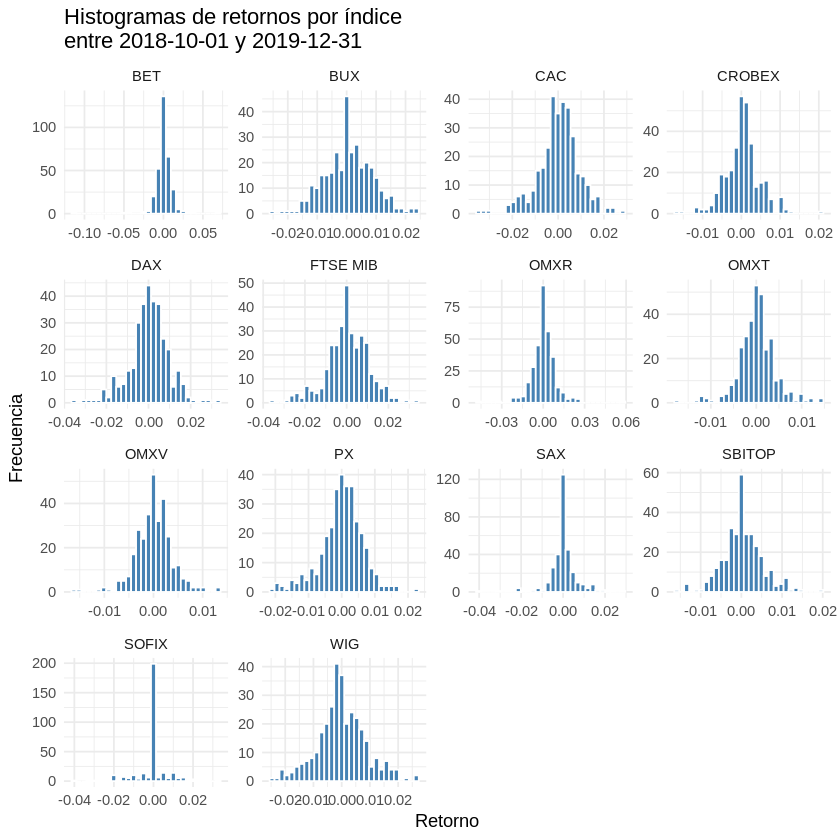
\includegraphics[width=\linewidth]{histograma.png}
    \end{minipage}
    \hfill
    \begin{minipage}{0.48\textwidth}
        \centering
        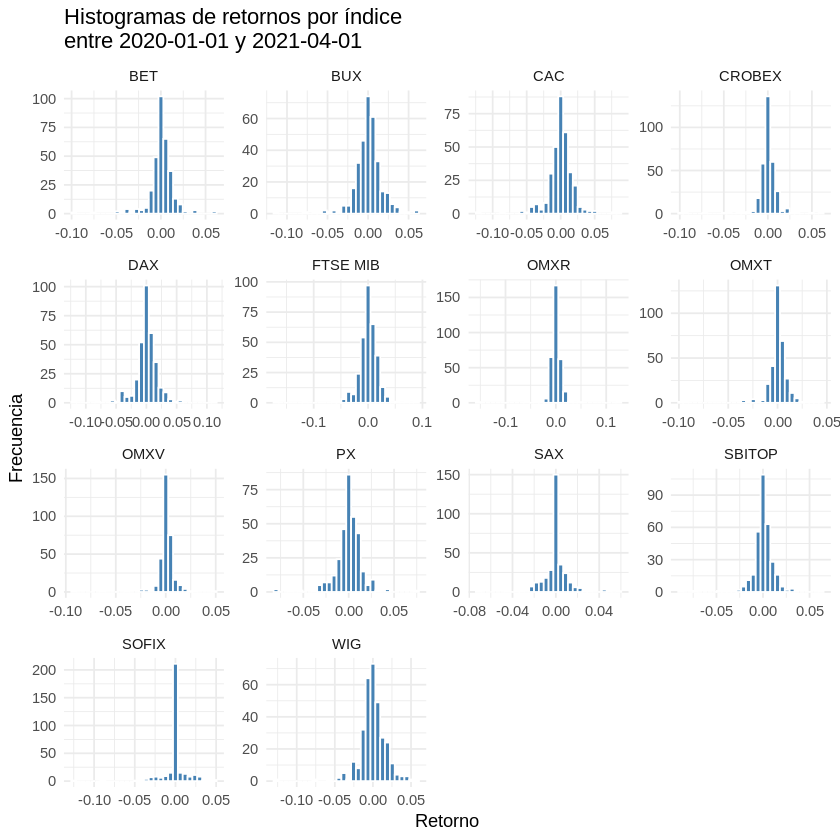
\includegraphics[width=\linewidth]{histograma2.png}
    \end{minipage}
    \caption{Histogramas de los retornos en distintos índices}
\end{figure}

\item Datos exploratorios: Boxplots
\begin{figure}[H]
    \centering
    \begin{minipage}{0.48\textwidth}
        \centering
        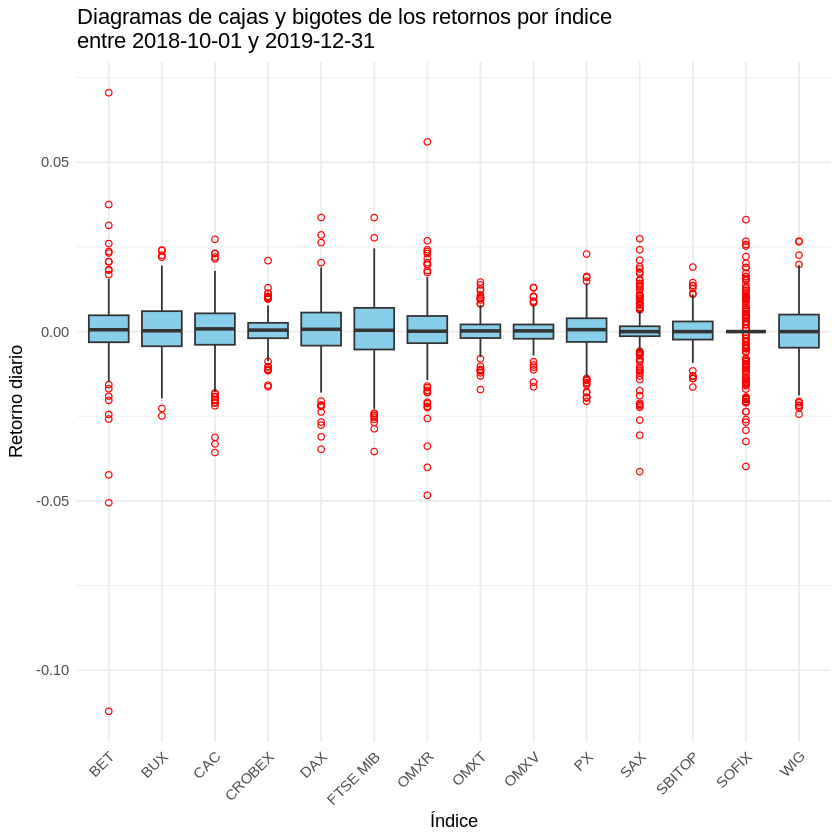
\includegraphics[width=\linewidth]{boxplots.png}
    \end{minipage}
    \hfill
    \begin{minipage}{0.48\textwidth}
        \centering
        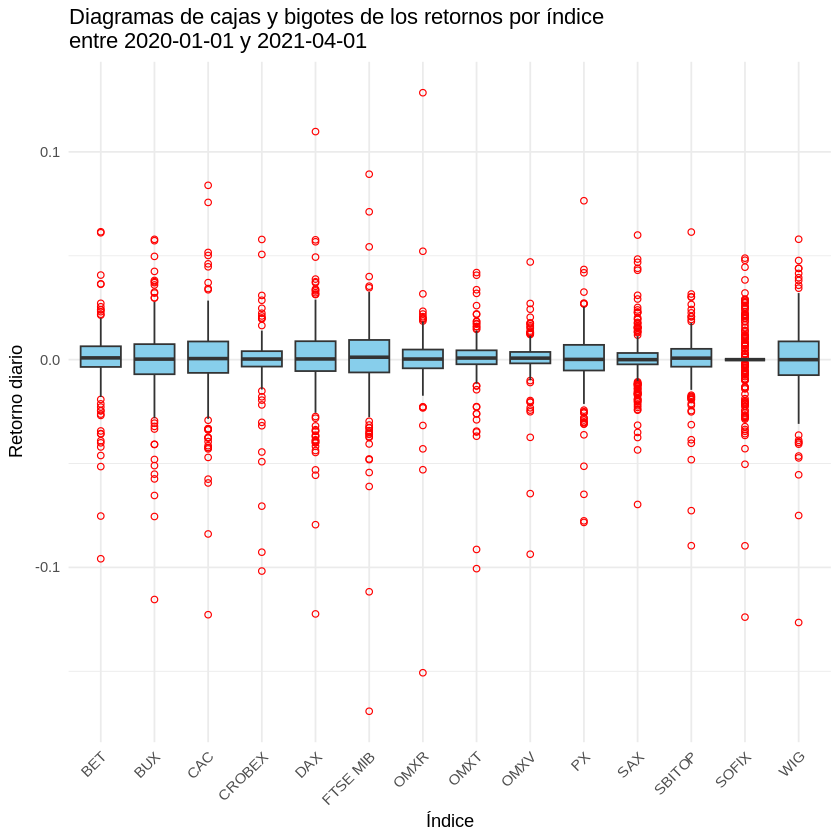
\includegraphics[width=\linewidth]{boxplots2.png}
    \end{minipage}
    \caption{Diagramas de caja comparando la dispersión de retornos}
\end{figure}

\item Datos exploratorios: QQ-plots
\begin{figure}[H]
    \centering
    \begin{minipage}{0.48\textwidth}
        \centering
        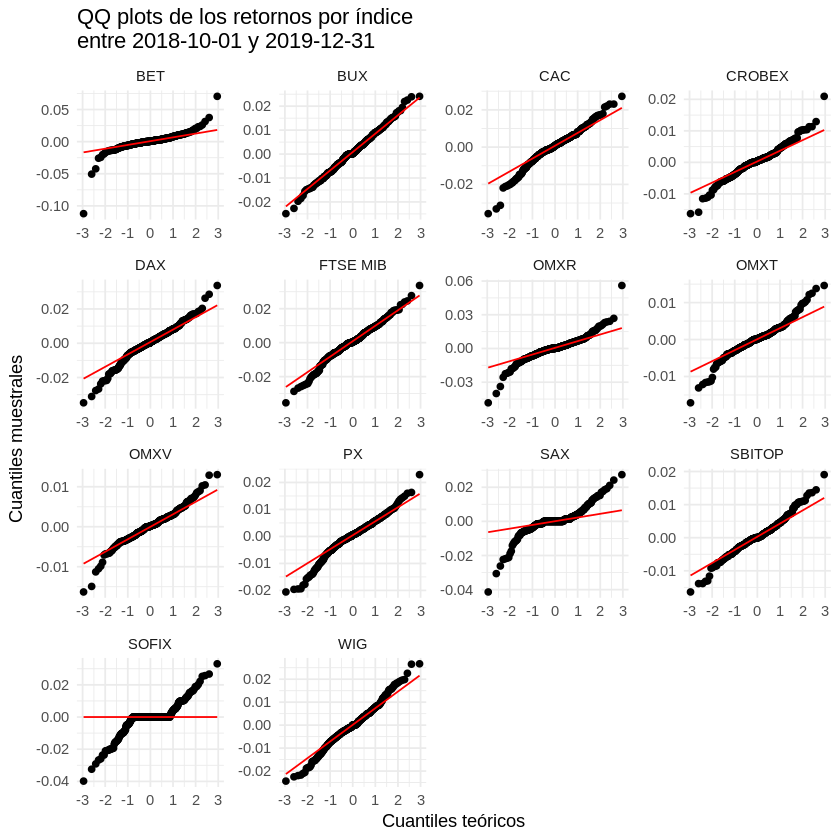
\includegraphics[width=\linewidth]{QQplot.png}
    \end{minipage}
    \hfill
    \begin{minipage}{0.48\textwidth}
        \centering
        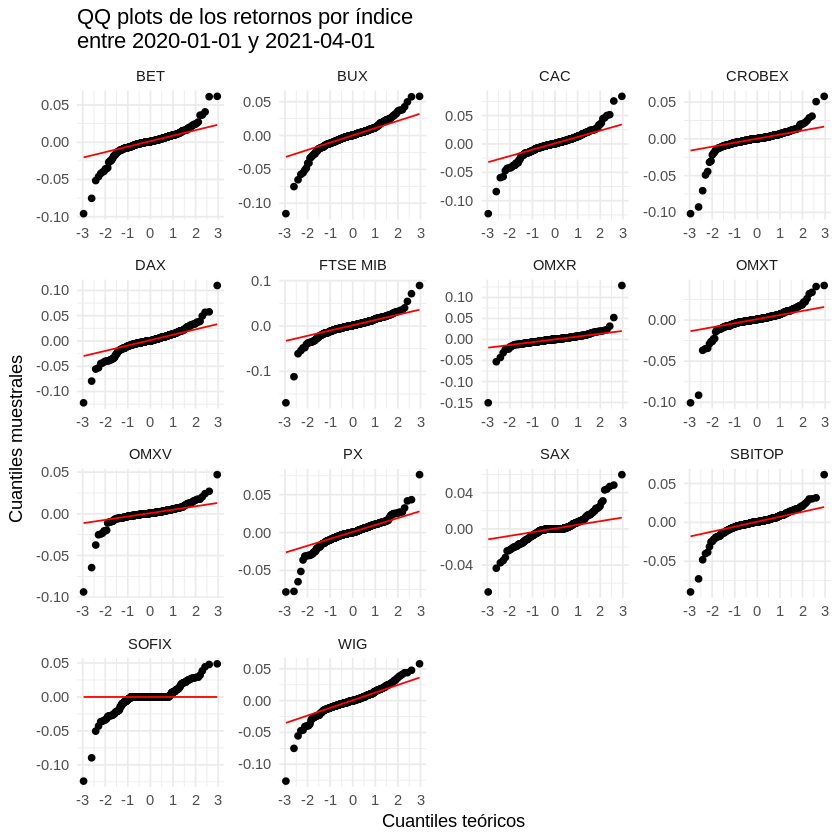
\includegraphics[width=\linewidth]{QQplot2.png}
    \end{minipage}
    \caption{QQ-plots para evaluar normalidad en los retornos}
\end{figure}
\end{itemize}

Como se aprecia, es necesario aplicar pruebas no paramétricas para series de tiempo ya que, en primera instancia, no hay evidencia por lo menos visual de que existe normalidad en los índices. Se aplicará más adelante prueba de normalidad Jarque-Bera para probar lo ultimamente dicho.

  \subsection {Cálculo de rendimientos logarítmicos diarios.}
  


\begin{table}[H]
\centering
\small
\caption{Resumen de retornos pre-COVID con datos propios}
\begin{tabular}{|l|r|r|r|r|r|r|r|}
\hline
\textbf{Índice} & \textbf{Media (\%)} & \textbf{Máx (\%)} & \textbf{Mín (\%)} & \textbf{Asimetría} & \textbf{Curtosis*} & \textbf{JB p-valor} & \textbf{AD p-valor} \\
\hline
BET     & 0.0588  &  7.0546 & -11.2121 & -2.5287 & 33.9003 & 0.0000     & 3.70e-24 \\
BUX     & 0.0727  &  2.4109 & -2.4893  &  0.0220 & 0.2112  & 7.33e-01   & 4.42e-01 \\
CAC     & 0.0296  &  2.7243 & -3.5702  & -0.5068 & 1.6108  & 3.02e-11   & 4.30e-06 \\
CROBEX  & 0.0398  &  2.0950 & -1.6283  &  0.0448 & 2.1349  & 5.48e-14   & 2.09e-06 \\
DAX     & 0.0264  &  3.3699 & -3.4755  & -0.3589 & 1.5310  & 4.97e-09   & 2.94e-06 \\
FTSE MIB& 0.0460  &  3.3669 & -3.5433  & -0.2680 & 0.8818  & 8.07e-04   & 9.56e-04 \\
OMXR    & 0.0230  &  5.6044 & -4.8341  & -0.0879 & 7.5479  & 0.0000     & 7.11e-17 \\
OMXT    & 0.0161  &  1.4632 & -1.7126  & -0.1065 & 2.6499  & 0.0000     & 1.08e-09 \\
OMXV    & 0.0127  &  1.3028 & -1.6311  & -0.2264 & 2.5654  & 0.0000     & 2.41e-05 \\
PX      & 0.0070  &  2.2896 & -2.0577  & -0.4419 & 1.2283  & 2.24e-07   & 6.13e-07 \\
SAX     & 0.0227  &  2.7380 & -4.1353  & -0.8305 & 7.3750  & 0.0000     & 3.70e-24 \\
SBITOP  & 0.0311  &  1.9057 & -1.6391  &  0.1547 & 1.3253  & 4.17e-06   & 2.29e-05 \\
SOFIX   & -0.0557 &  3.3066 & -3.9823  & -0.5191 & 3.9519  & 0.0000     & 3.70e-24 \\
WIG     & -0.0023 &  2.6705 & -2.4379  &  0.0585 & 0.5759  & 9.93e-02   & 1.87e-03 \\
\hline
\end{tabular}
\end{table}



\begin{table}[H]
\centering
\small
\caption{Resumen de retornos post-COVID con datos propios}
\begin{tabular}{|l|r|r|r|r|r|r|r|}
\hline
\textbf{Índice} & \textbf{Media (\%)} & \textbf{Máx (\%)} & \textbf{Mín (\%)} & \textbf{Asimetría} & \textbf{Curtosis*} & \textbf{JB p-valor} & \textbf{AD p-valor} \\
\hline
BET     & 0.0495  & 6.1546  & -9.5844  & -1.4233 & 11.7880 & 0.0000     & 3.70e-24 \\
BUX     & 0.0027  & 5.7900  & -11.5457 & -1.2546 & 8.1332  & 0.0000     & 1.82e-18 \\
CAC     & 0.0237  & 8.3895  & -12.2768 & -0.9396 & 9.0701  & 0.0000     & 3.52e-22 \\
CROBEX  & -0.0142 & 5.7840  & -10.1764 & -3.0968 & 25.9527 & 0.0000     & 3.70e-24 \\
DAX     & 0.0585  & 10.9759 & -12.2386 & -0.6197 & 9.7628  & 0.0000     & 8.57e-23 \\
FTSE MIB& 0.0361  & 8.9256  & -16.9238 & -2.2363 & 19.4570 & 0.0000     & 1.82e-23 \\
OMXR    & 0.0353  & 12.8473 & -15.0709 & -1.4794 & 56.7660 & 0.0000     & 3.70e-24 \\
OMXT    & 0.0577  & 4.1911  & -10.0598 & -3.5146 & 30.2955 & 0.0000     & 3.70e-24 \\
OMXV    & 0.0600  & 4.7005  & -9.3655  & -3.9268 & 38.9397 & 0.0000     & 3.70e-24 \\
PX      & 0.0040  & 7.6475  & -7.8364  & -0.8807 & 8.1263  & 0.0000     & 3.23e-19 \\
SAX     & 0.0177  & 5.9964  & -6.9707  & 0.1042  & 7.8704  & 0.0000     & 3.70e-24 \\
SBITOP  & 0.0296  & 6.1401  & -8.9558  & -1.8640 & 15.6632 & 0.0000     & 3.70e-24 \\
SOFIX   & -0.0239 & 4.8840  & -12.3932 & -2.2810 & 18.2041 & 0.0000     & 3.70e-24 \\
WIG     & 0.0189  & 5.7954  & -12.6516 & -1.3540 & 9.8830  & 0.0000     & 1.69e-14 \\
\hline
\end{tabular}
\end{table}

 \subsection{Conclusiones sobre forma de distribución}

Al comparar los indicadores de forma de los retornos en los periodos pre y post-COVID, se identifican patrones consistentes:

\begin{itemize}
    \item \textbf{Asimetría:} en ambos periodos predominan asimetrías negativas, pero estas se intensifican tras la pandemia. Índices como CROBEX, OMXV y OMXT presentan valores absolutos mayores a 3, lo que sugiere colas más pesadas hacia extremos negativos.
    
    \item \textbf{Curtosis excesiva:} los valores de curtosis aumentan significativamente en el periodo post-COVID, en algunos casos superando 30 o incluso 50. Esto indica una mayor concentración de eventos extremos y mayor propensión a choques bruscos en los precios.
    
    \item \textbf{Normalidad:} las pruebas de Jarque-Bera y Anderson-Darling muestran p-valores cercanos a cero en casi todos los índices, particularmente en el periodo post-COVID, lo que confirma la no normalidad de los retornos en ambos periodos, pero con mayor intensidad post-pandemia.
\end{itemize}

En resumen, los retornos diarios muestran una distribución más sesgada, con colas pesadas y presencia de eventos extremos más frecuentes tras el inicio del COVID-19, lo que justifica el uso de pruebas no paramétricas en el análisis de eficiencia de mercado.


\subsection {Aplicación de las prueba: Runs Test, Bartels y Wright (R1, R2, S1).}

\subsubsection{\large Runs Test}

$H_0$: Los datos son independientes (las observaciones siguen una secuencia aleatoria).\\
$H_1$: Los datos no son independientes (existe patrón o dependencia en la secuencia de signos).\\

Se aplica a secuencias binarias (como signos positivos/negativos) para detectar aleatoriedad.

\begin{table}[H]
\centering
\small
\caption{Los p-valor de Runs Test a los retornos pre-COVID con datos propios}
\begin{tabular}{|l|r|r|r|r|r|r|r|}
\hline
\textbf{Index} & \textbf{Runs Test Z} & \textbf{p-value} & \textbf{Reject $H_0$ (i.i.d)} \\
\hline
BET & 0.5872 & 0.5571 & No \\
BUX & 0.1763 & 0.8600 & No \\
CAC & -1.3264 & 0.1847 & No \\
CROBEX & -0.1884 & 0.8506 & No \\
DAX & -0.4894 & 0.6246 & No \\
FTSE MIB & -0.2656 & 0.7905 & No \\
OMXR & 3.5237 & 0.0004 & Yes \\
OMXT & -0.2505 & 0.8022 & No \\
OMXV & -2.0497 & 0.0404 & Yes \\
PX & -2.0126 & 0.0442 & Yes \\
SAX & -0.0196 & 0.9843 & No \\
SBITOP & -0.7132 & 0.4757 & No \\
SOFIX & 0.7098 & 0.4778 & No \\
WIG & 0.0913 & 0.9273 & No \\
\hline
\end{tabular}
\end{table}

\begin{table}[H]
\centering
\small
\caption{Los p-valor de Runs Test a los retornos post-COVID con datos propios}
\begin{tabular}{|l|r|r|r|r|r|r|r|}
\hline
\textbf{Index} & \textbf{Runs Test Z} & \textbf{p-value} & \textbf{Reject $H_0$ (i.i.d)} \\
\hline
BET & -1.9138 & 0.0556 & No \\
BUX & -0.2785 & 0.7807 & No \\
CAC & 1.2369 & 0.2161 & No \\
CROBEX & 0.9621 & 0.3360 & No \\
DAX & 1.6208 & 0.1051 & No \\
FTSE MIB & 0.6519 & 0.5144 & No \\
OMXR & 2.0714 & 0.0383 & Yes \\
OMXT & -3.0202 & 0.0025 & Yes \\
OMXV & -0.1809 & 0.8565 & No \\
PX & -0.8358 & 0.4033 & No \\
SAX & 2.6668 & 0.0077 & Yes \\
SBITOP & -0.5423 & 0.5876 & No \\
SOFIX & -0.8835 & 0.3770 & No \\
WIG & 0.9621 & 0.3360 & No \\
\hline
\end{tabular}
\end{table}


El Runs Test permite evaluar si una serie temporal presenta independencia entre observaciones sucesivas, es decir, si los retornos son aleatorios (i.i.d). Al comparar los resultados pre y post COVID-19, se observan los siguientes hallazgos relevantes:

\begin{itemize}

\item \textbf {Estabilidad en la aleatoriedad:} La mayoría de los índices mantienen una estructura similar en cuanto a la independencia de los retornos antes y después del COVID-19, ya que en ambos periodos no se rechaza la hipótesis nula de aleatoriedad. Ejemplos de ello son los índices BET, BUX, CAC, CROBEX, DAX, FTSE MIB, SBITOP, SOFIX y WIG.

\item \textbf  {Cambio en la aleatoriedad (ruptura estructural):} Algunos índices muestran un cambio significativo en su comportamiento post-COVID.OMXT y SAX, que no mostraban evidencia de dependencia en el periodo previo, pasan a rechazar la hipótesis nula en el periodo posterior, lo que indica que sus retornos dejaron de comportarse de forma aleatoria.El caso inverso se presenta en OMXV y PX, donde se rechazaba la aleatoriedad en el periodo previo, pero no después.\\

\item \textbf  {Persistencia de no aleatoriedad:} El índice OMXR rechaza la hipótesis de aleatoriedad en ambos periodos, lo que sugiere una estructura no aleatoria persistente, posiblemente relacionada con factores estructurales propios de ese mercado.

\end{itemize}   


\subsubsection {\large Test de Bartels (versión de rangos del test de Von Neumann)}

$H_0$: Los datos son independientes e idénticamente distribuidos (i.i.d.).\\
$H_1$: Los datos no son independientes (existe dependencia secuencial).\\

Este test detecta autocorrelación sin asumir normalidad, usando los rangos de los datos.

\begin{table}[H]
\centering
\small
\caption{Resultados del Test de Bartels (pre-COVID vs post-COVID)}
\begin{tabular}{|l|r|r|c|r|r|c|}
\hline
\textbf{Índice} & \multicolumn{3}{c|}{\textbf{Pre-COVID}} & \multicolumn{3}{c|}{\textbf{Post-COVID}} \\
\cline{2-7}
 & \textbf{Z} & \textbf{p-valor} & \textbf{Rechaza $H_0$} & \textbf{Z} & \textbf{p-valor} & \textbf{Rechaza $H_0$} \\
\hline
BET       & -0.4667 & 0.6407 & No  & -2.1257 & 0.0335 & Sí \\
BUX       & -0.4600 & 0.6455 & No  & -0.5733 & 0.5664 & No \\
CAC       & -0.1579 & 0.8746 & No  &  0.6895 & 0.4905 & No \\
CROBEX    & -0.4183 & 0.6757 & No  & -0.4775 & 0.6330 & No \\
DAX       &  0.2619 & 0.7934 & No  &  1.2574 & 0.2086 & No \\
FTSE MIB  &  0.3530 & 0.7241 & No  &  0.8446 & 0.3983 & No \\
OMXR      &  4.1703 & 0.0000 & Sí  &  4.0750 & 0.0000 & Sí \\
OMXT      &  0.4406 & 0.6595 & No  & -3.5593 & 0.0004 & Sí \\
OMXV      & -3.2453 & 0.0012 & Sí  & -1.7172 & 0.0859 & No \\
PX        & -1.2422 & 0.2142 & No  & -1.4834 & 0.1379 & No \\
SAX       &  1.4472 & 0.1478 & No  &  2.7447 & 0.0061 & Sí \\
SBITOP    & -0.2477 & 0.8043 & No  & -0.1969 & 0.8439 & No \\
SOFIX     &  1.7496 & 0.0802 & No  &  1.3044 & 0.1921 & No \\
WIG       &  0.3079 & 0.7582 & No  &  0.9724 & 0.3308 & No \\
\hline
\end{tabular}
\end{table}

\subsubsection {\large Test Wright en sus formulaciones R1, R2 y S1}


\begin{itemize}
\item {Hipótesis nula ($H_0$):} La serie temporal sigue un paseo aleatorio. Es decir, los incrementos son independientes e idénticamente distribuidos (IID) con media cero y varianza constante.\\

\item {Hipótesis alternativa ($H_1$):}La serie NO sigue un paseo aleatorio. Puede existir dependencia serial o heterocedasticidad (varianza no constante) en los incrementos.\\
\end{itemize}


{\large Estadísticos del test:}

\begin{itemize}
\item R1 : basado en los rangos de los incrementos, detecta dependencias en la estructura de la serie.

\item R2 : basado en la combinación de rangos y signos, sensible a ciertas formas de dependencia que los tests clásicos no capturan.

\item S1 : basado en los signos de los incrementos, útil para detectar asimetrías o dependencia en la dirección de los cambios.

\end{itemize}

Para ver los resultados extensos vease del jupiter anexo a la carpeta de este documento


\section{Comparación de resultados}
En general, los resultados obtenidos con nuestro código fueron consistentes con los hallazgos de Iordache. Por ejemplo, se confirmó que los mercados desarrollados (Francia, Alemania e Italia) no mostraron evidencias claras de ineficiencia, mientras que los mercados emergentes presentaron respuestas más heterogéneas, especialmente Letonia y Lituania.

\begin{table}[H]
\centering
\begin{tabular}{|l|c|c|}
\hline
\textbf{Índice} & \textbf{Artículo Original} & \textbf{Reproducción}\\
\hline
CAC 40 (Francia) & EMH válida & EMH válida\\
OMXT (Estonia) & EMH post-COVID rechazada & EMH post-COVID rechazada\\
OMXR (Letonia) & EMH rechazada & EMH rechazada\\
BUX (Hungría) & EMH válida & EMH válida\\
BET (Rumanía) & EMH pre-COVID válida, post rechazada & Coincidente\\
\hline
\end{tabular}
\caption{Comparación resumida entre resultados originales y reproducidos}
\end{table}

\section{Conclusiones}
La simulación realizada permitió confirmar gran parte de los hallazgos del artículo original. Las pruebas no paramétricas utilizadas fueron efectivas incluso usando una fuente de datos diferente, reforzando la robustez metodológica del estudio. Este ejercicio también destaca la relevancia de reproducir estudios empíricos como forma de validación científica.

\section*{Referencias}
\begin{itemize}
  \item Iordache, A. (2024). Market Efficiency During the COVID-19 Pandemic. Eastern European Economics 62(2), 136–164.
  \item Wright, J.H. (2000). Alternative Variance-Ratio Tests Using Ranks and Signs. Journal of Business \& Economic Statistics.
  \item Bartels, R. (1982). The Rank Version of von Neumann’s Ratio Test for Randomness. JASA.
  \item Wald, A. \& Wolfowitz, J. (1940). On a Test Whether Two Samples are from the Same Population.
\end{itemize}

\end{document}

